
\section{Old stuff}

The operation to be performed is given by a sequence of vectors
\be\label{eq:weight_P}
p^{(t)}_i = \sigma( P_i h^{(t-1)} ) \in \mathbb{R}^{n_P}\,, 1 \le i \le m
\ee
in a way that we will now explain. In outline, we think of the entries of $p^{(t)}_i$ as telling us the coefficients of monomials in the entries of $x^{(t)}$ and $h^{(t-1)}$ to use in the modified update equation. For simplicity let us only consider monomials of degree $2$ in what follows, since the general case is similar. We set
\be\label{eq:weight_E}
y^{(t)} = E x^{(t)} \oplus h^{(t-1)} \in \mathbb{R}^{n_Y}
\ee
where $E$ is another matrix of weights. See Example \ref{??} for an explanation.

Let $F$ denote a linear map $F: M_{n_Y}(\mathbb{R}) \lto \mathbb{R}^{n_Y^2}$ which reads off the entries of a matrix into a column vector. In TensorFlow we can represent this using \emph{reshape}. Writing $Y = y^{(t)}$ observe that $Y Y^T$ is an $n_Y \times n_Y$ matrix with $(i,j)$-entry $Y_i Y_j$. We choose $n_P = n_Y^2$ and compute the entry-wise multiplication
\[
p^{(t)}_i \odot F(Y Y^T) = p^{(t)}_i \odot F\big( y^{(t)} ( y^{(t)} )^T \big) \in \mathbb{R}^{n_P}\,.
\]
Finally, $q^{(t)}$ is the column vector whose $i$th row is $p^{(t)}_i \odot F(Y Y^T)$, that is,
\[
q^{(t)} = \begin{pmatrix} p^{(t)}_1 \odot F\big( y^{(t)} ( y^{(t)} )^T \big) \\
\vdots\\
p^{(t)}_m \odot F\big( y^{(t)} ( y^{(t)} )^T \big) \end{pmatrix}\,.
\] 
In summary, we view $x^{(t)}, h^{(t-1)}$ as respectively the differentiable analogues of \verb+A,R2+ and the sequence $p^{(t)}_1, \ldots, p^{(t)}_m$ as the analogue of the command \verb+ADD+. The output of the command is the vector $q^{(t)}$. We incorporate this output into the update equation as follows:
\be\label{eq:final_update}
h^{(t+1)} = \sigma\big( V q^{(t)} + H h^{(t)} + U x^{(t+1)} \big)\,.
\ee
Thus $V$ is the differentiable analogue of the register \verb+R3+. The weights are $P_i$ from \eqref{eq:weight_P}, $E$ from \eqref{eq:weight_E} and $V, H, U$ from \eqref{eq:final_update}. This architecture is easily generalised to polynomials of higher degree, by adding additional terms.

\begin{example} Let us consider how the system might reproduce the program that repeats every digit of an input binary sequence, e.g.
\be\label{eq:approx_map}
0110 \longmapsto 00111100\,.
\ee
We take the inputs $x \in \mathbb{R}^2$ with $e_1 = (1,0)$ standing for the binary digit $1$ and $e_0 = (0,1)$ standing for $0$. We suppose that the system has learned the embedding matrix $E$ such that $A = E(e_1)$ and $B = E(e_0)$ are matrices in $M_n(\mathbb{R}_{>0})$ with the property that the subgroup they generate under multiplication is a free group on two letters. This condition just means that the map
\[
\Psi: \{0,1\}^* \lto M_n( \mathbb{R} )
\]
from binary sequences to matrices, defined inductively for $s \in \{0,1\}$ by
\[
\Psi( s S ) = \begin{cases} B \Psi(S) & s = 0 \\ A \Psi(S) & s = 1 \end{cases}
\]
is injective. The space of matrices $\mathscr{H} = M_n(\mathbb{R})$ is the internal state of our RNN. To extract output from the RNN we apply a series of fully-connected layers with the final internal state $h^{(T)}$ as input, and we think of this series of layers as approximating a function $\Psi': M_n(\mathbb{R}) \lto \{0,1\}^*$ with the property that $\Psi' \circ \Psi = 1$, that is, which can read off from a product of matrices $ABA$ the corresponding binary sequence $101$. So, in order to approximate the function \eqref{eq:approx_map} our RNN needs to take the inputs
\[
x^{(1)} = B, x^{(2)} = A, x^{(3)} = A, x^{(4)} = B
\]
and produce the final internal state
\[
h^{(T)} = BBAAAABB \in M_n(\mathbb{R})\,.
\]
This can be be done if we assume that in the update equation \eqref{eq:final_update} has weights $H, U = 0$ and $V$ is chosen so that
\[
V q^{(t)} = (x^{(t)})^2 h^{(t-1)}\,.
\]
Note that the right hand side is a cubic polynomial in the entries of $x^{(t)}, h^{(t-1)}$ so we actually need the generalised form of \eqref{eq:final_update}.
\end{example}

\begin{example}[(Stack-augmented RNN)] Thinking of an RNN as a state machine automata, and by analogy with a pushdown automata, an RNN can be augmented with an external stack memory \cite{highorderrec}. We can emulate the more recent version of this idea in \cite{joulin} with appropriate choices of the defining data of the LLRNN. We begin with a decomposition of the hidden state space as $\mathscr{H} = \mathscr{H}_0 \oplus \mathscr{S}$ where the ``memory stack''
\be
\mathscr{S} = k[z]/z^{N+1} = k1 \oplus kz \oplus \cdots \oplus kz^N
\ee
is equipped with the push and pop operators $p_{+},p_{-}: \mathscr{S} \lto \mathscr{S}$ with matrices
\[
p_{+} = \begin{pmatrix} 0 & 0 & \cdots & 0 & 0 \\
1 & 0 & \cdots & 0 & 0 \\
0 & 1 & \cdots & 0 & 0\\
\vdots & & \ddots & & \vdots \\
0 & 0 & \cdots & 1 & 0\\
\end{pmatrix}\,,\qquad
p_{-} = \begin{pmatrix} 0 & 1 & 0 & \cdots & 0 \\
0 & 0 & 1 & \cdots & 0 \\
\vdots &  &  & \ddots & \vdots \\
0 & 0 & 0 & \cdots & 1\\
0 & 0 & 0 & \cdots & 0
\end{pmatrix}\,.
\]
We also constrain the weight matrix $H$ to be of the form
\[
H = \begin{pmatrix} H_0 & 0 \\ 0 & 0 \end{pmatrix}
\]
with respect to the direct sum decomposition $\mathscr{H} = \mathscr{H}_0 \oplus \mathscr{S}$. 

The master program is a proof (which we omit) of
\be
{!}1, \,{!}( \inta_A \oplus \inta_A ), \,{!}(S \multimap S), \,{!}(S \multimap S) \vdash A \multimap A
\ee
with the property that $\den{S} = \mathscr{S}$ and
\[
\den{\master}_{nl}(\tau, \den{\underline{m}} \oplus \den{\underline{n}}, \alpha, \beta ) = \tau J(1) + J \circ \alpha^m \circ \beta^n \circ I\,,
\]
where $I: \mathscr{H} \lto \mathscr{S}$ and $J: \mathscr{S} \lto \mathscr{H}$ are the projections and injections respectively. We note that for $\lambda, \mu \in k$
\[
\den{\master}_{nl}( \tau, \lambda\den{\underline{1}} \oplus \den{\underline{0}} + \mu \den{\underline{0}} \oplus \den{\underline{1}}, \alpha, \beta ) = \tau J(1) + \lambda J \circ \alpha \circ I + \mu J \circ \beta \circ I\,.
\]
The command types are $P_1 = 1, P_2 = \inta_A \oplus \inta_A$ and the input types are $B_1 = B_2 = S$. We take $\mathscr{B}_j = \End_{\mathbb{R}}(\mathscr{S})$ for $j \in \{1,2\}$, $\mathscr{P}_1 = k$ and
\be
\mathscr{P}_2 = \operatorname{span}( \den{\underline{1}} \oplus \den{\underline{0}}, \den{\underline{0}} \oplus \den{\underline{1}} ) \subseteq \den{\inta_A} \oplus \den{\inta_A}\,.
\ee
We assume the weight matrices $V_j$ are fixed during training with the image of every basis element equal to $p_{+}$ for $j = 1$ and $p_{-}$ for $j = 2$. 

Now let us explain why this emulates a stack-based memory. At time $t$, we write
\[
h^{(t)} = (h_0^{(t)}, s^{(t)})^T
\]
and view $h_0^{(t)}$ as the internal state of the RNN and $s^{(t)} = (s_0^{(t)}, \ldots, s_N^{(t)})^T$ as the contents of the stack at time $t$. Suppose that the command vectors generated by the controller are the scalar $W_1(h^{(t)}) \in k$ and
\[
W_2(h^{(t)}) = \lambda \den{\underline{1}} \oplus \den{\underline{0}} + \mu \den{\underline{0}} \oplus \den{\underline{1}}
\]
for some $\lambda,\mu \in k$.
Then with $\alpha = p_{+}$ and $\beta = p_{-}$ and  we have
\begin{align*}
H h^{(t)} + Z &= J\den{\master}_{nl}\big( W_1(h^{(t)}), W_2(h^{(t)}), p_+, p_-\big)I( h^{(t)} )\\
&= H h^{(t)} + W_1(h^{(t)}) J(1) + J\big( \lambda p_+ + \mu p_{-} \big)I( h_0^{(t)}, s^{(t)})^T\\
&= H h^{(t)} + J\begin{pmatrix} W_1(h^{(t)}) + \mu s_1^{(t)}, & \lambda s_0^{(t)} + \mu s_2^{(t)}, & \cdots, & \lambda s_{N-1}^{(t)} \end{pmatrix}^T\\
&= \begin{pmatrix}
H_0 h_0^{(t)}, &
W_1(h^{(t)}) + \mu s_1^{(t)}, & 
\lambda s_0^{(t)} + \mu s_2^{(t)},
\cdots,\,
\lambda s_{N-1}^{(t)}
\end{pmatrix}
\end{align*}
which agrees with the hidden state of the stack-augmented RNN \cite{joulin} with hidden-to-hidden weight matrix $H_0$, after it has predicted with probability $\lambda$ to push $W_1(h^{(t)})$ onto the stack, and with probability $\mu$ to pop the stack. To store vectors in a vector space $V$ rather than a scalar at each stack position, we simply replace $\mathscr{S}$ by $\mathscr{S} \otimes V$.
\end{example}

\section{Background on CPUs}\label{section:appendix_cpu}

Recall that an assembly program for an ordinary CPU looks like
\begin{verbatim}
LOAD R1, A
ADD R3, R1, R2
STORE C, R3
\end{verbatim}
Where \verb+R1,R2,R3+ stand for the first three registers of the CPU and \verb+A,B,C+ are numbers representing addresses in memory. Thus series of instructions will result in the CPU fetching a number from memory location \verb+A+ and storing it in \verb+R1+, adding this number to a previously stored number in \verb+R2+ with the result being stored in \verb+R3+, and finally writing that register out to the memory address \verb+C+. In the analogy between a CPU and a vanilla RNN we think of the number read from \verb+A+ as the current input $x^{(t)}$ and the previously stored value in \verb+R2+ as (part of) the internal state $h^{(t-1)}$.

Recent work \cite{??,??} on coupling memory to neural networks takes as its starting point the first of the above instructions \verb+LOAD R1, A+ and makes it ``differentiable'' by having the RNN controller predict at time $t$ both the memory address \verb+A+ and the register \verb+R3+ to write to (in this case for example, as a mask on the vector giving the internal state $h^{(t+1)}$). The same differentiable interpretation can be given of the \verb+STORE+ command. This is done by adding suitable terms to the update equation \eqref{eq:update_eqn}.

In contrast our focus is on the third command, the \verb+ADD+. We increase the expressive power of the update equation by allowing it to predict at time $t$ an operation $p^{(t)}$ (a vector specifying a point in a space of ``programs'') which is to be performed on the input and internal state. In order to preserve our analogy with CPU instructions even without \verb+LOAD+ and \verb+STORE+, we could imagine a CPU with a command
\begin{verbatim}
ADD R3, A, R2
\end{verbatim}
which at once reads the number from address \verb+A+, adds it to the stored value in \verb+R2+ and writes the result to \verb+R3+. Note that without a \verb+LOAD+ instruction, the only way a value could have gotten into \verb+R2+ in a previous time step is as the result of another \verb+ADD+.

%\begin{remark} Although the architecture takes some inspiration from normal CPUs, there is an important distinction: on a normal CPU the program is given as a series of instructions prior to the beginning of execution. In contrast, in the model we have described each command is \emph{predicted} at runtime from the current internal state. Perhaps we can understand the process intuitively as follows: we are co-learning a part of $H$, call it $H_0$, which generates some part of the internal state $h^{(1)}_{0}, h^{(2)}_{0}, \ldots$ giving a path through the state space on which the weight matrix $P$ picks out the right program to run at each time step. The overall algorithm is distributed amongst the weights of $H_0$ and $P$.

%This also suggests an alternative algorithm: we do not predict $p^{(t)}$ at each time step, rather we have some fixed number of time steps $T$ and matrices of weights $p^{(1)}, \ldots, p^{(T)}$ which are learned by gradient descent.
%\end{remark}

\subsection{Old example}

We could add further memory rings to manipulate the read or write address of the first two memory rings, but this does not introduce anything essentially new. A more interesting demonstration of the underlying ideas of the coupling to linear logic is given in the next example, which adds two additional memory rings: the first stores constructions of \emph{new iterators from old ones} and the second stores \emph{iterators of these constructions}.

For any type $A$ and $n \ge 0$ there is a Church numeral $\underline{n}_A$ which is a proof of $\inta_A$. We have been omitting the subscript and writing $\underline{n}$ for this proof in the above, but in what follows we will need to sometimes reinstate the subscripts.

Consider memory rings with address space $\mathscr{W}$ and coefficient spaces
\[
\mathscr{V}_3 \subseteq \den{ \inta_{W} \multimap \inta_W }\,, \qquad \mathscr{V}_4 \subseteq \den{ \inta_{\inta_W} }
\]
which are spanned by denotations of linear logic proofs. Proofs of $\inta_W \multimap \inta_W$ construct new iterators from old ones, and since these iterators are naturally identified with integers, we are talking about functions $\mathbb{N} \lto \mathbb{N}$. For example, the proof $\pi_k = \underline{\mathrm{mult}}(k,-)$ of this type \cite[\S 6.1]{murfet_ll} has the property that
\begin{gather*}
\den{\pi_k}: \den{\inta_W} \lto \den{\inta_W}\,,\\
\den{\underline{m}_W} \longmapsto \den{\underline{mk}_W}\,.
\end{gather*}
Proofs of $\inta_{\inta_W}$ are iterators of proofs of the type $\inta_W \multimap \inta_W$. For instance, the proof $\underline{n}_{\inta_W}$ of $\inta_{\inta_W}$ applied to a proof $\rho$ of $\inta_W \multimap \inta_W$ returns this proof iterated $n$ times. In particular, $\underline{n}_{\inta_W}$ applied to $\pi_k$ returns $\pi_{k^n}$ \cite[Example 7.4]{murfet_ll}. The read addresses of these new rings allows the controller to specify that the chosen iterator from the second ring of the extended NTM be modified according to the selected proof in the third ring, and that this modification be iterated the number of times specified by the fourth ring.

Once again, let us first explain the dynamics induced by the additional memory rings with an example. Suppose at time $t = t_0$ the memory state of the first two rings is
\begin{center}
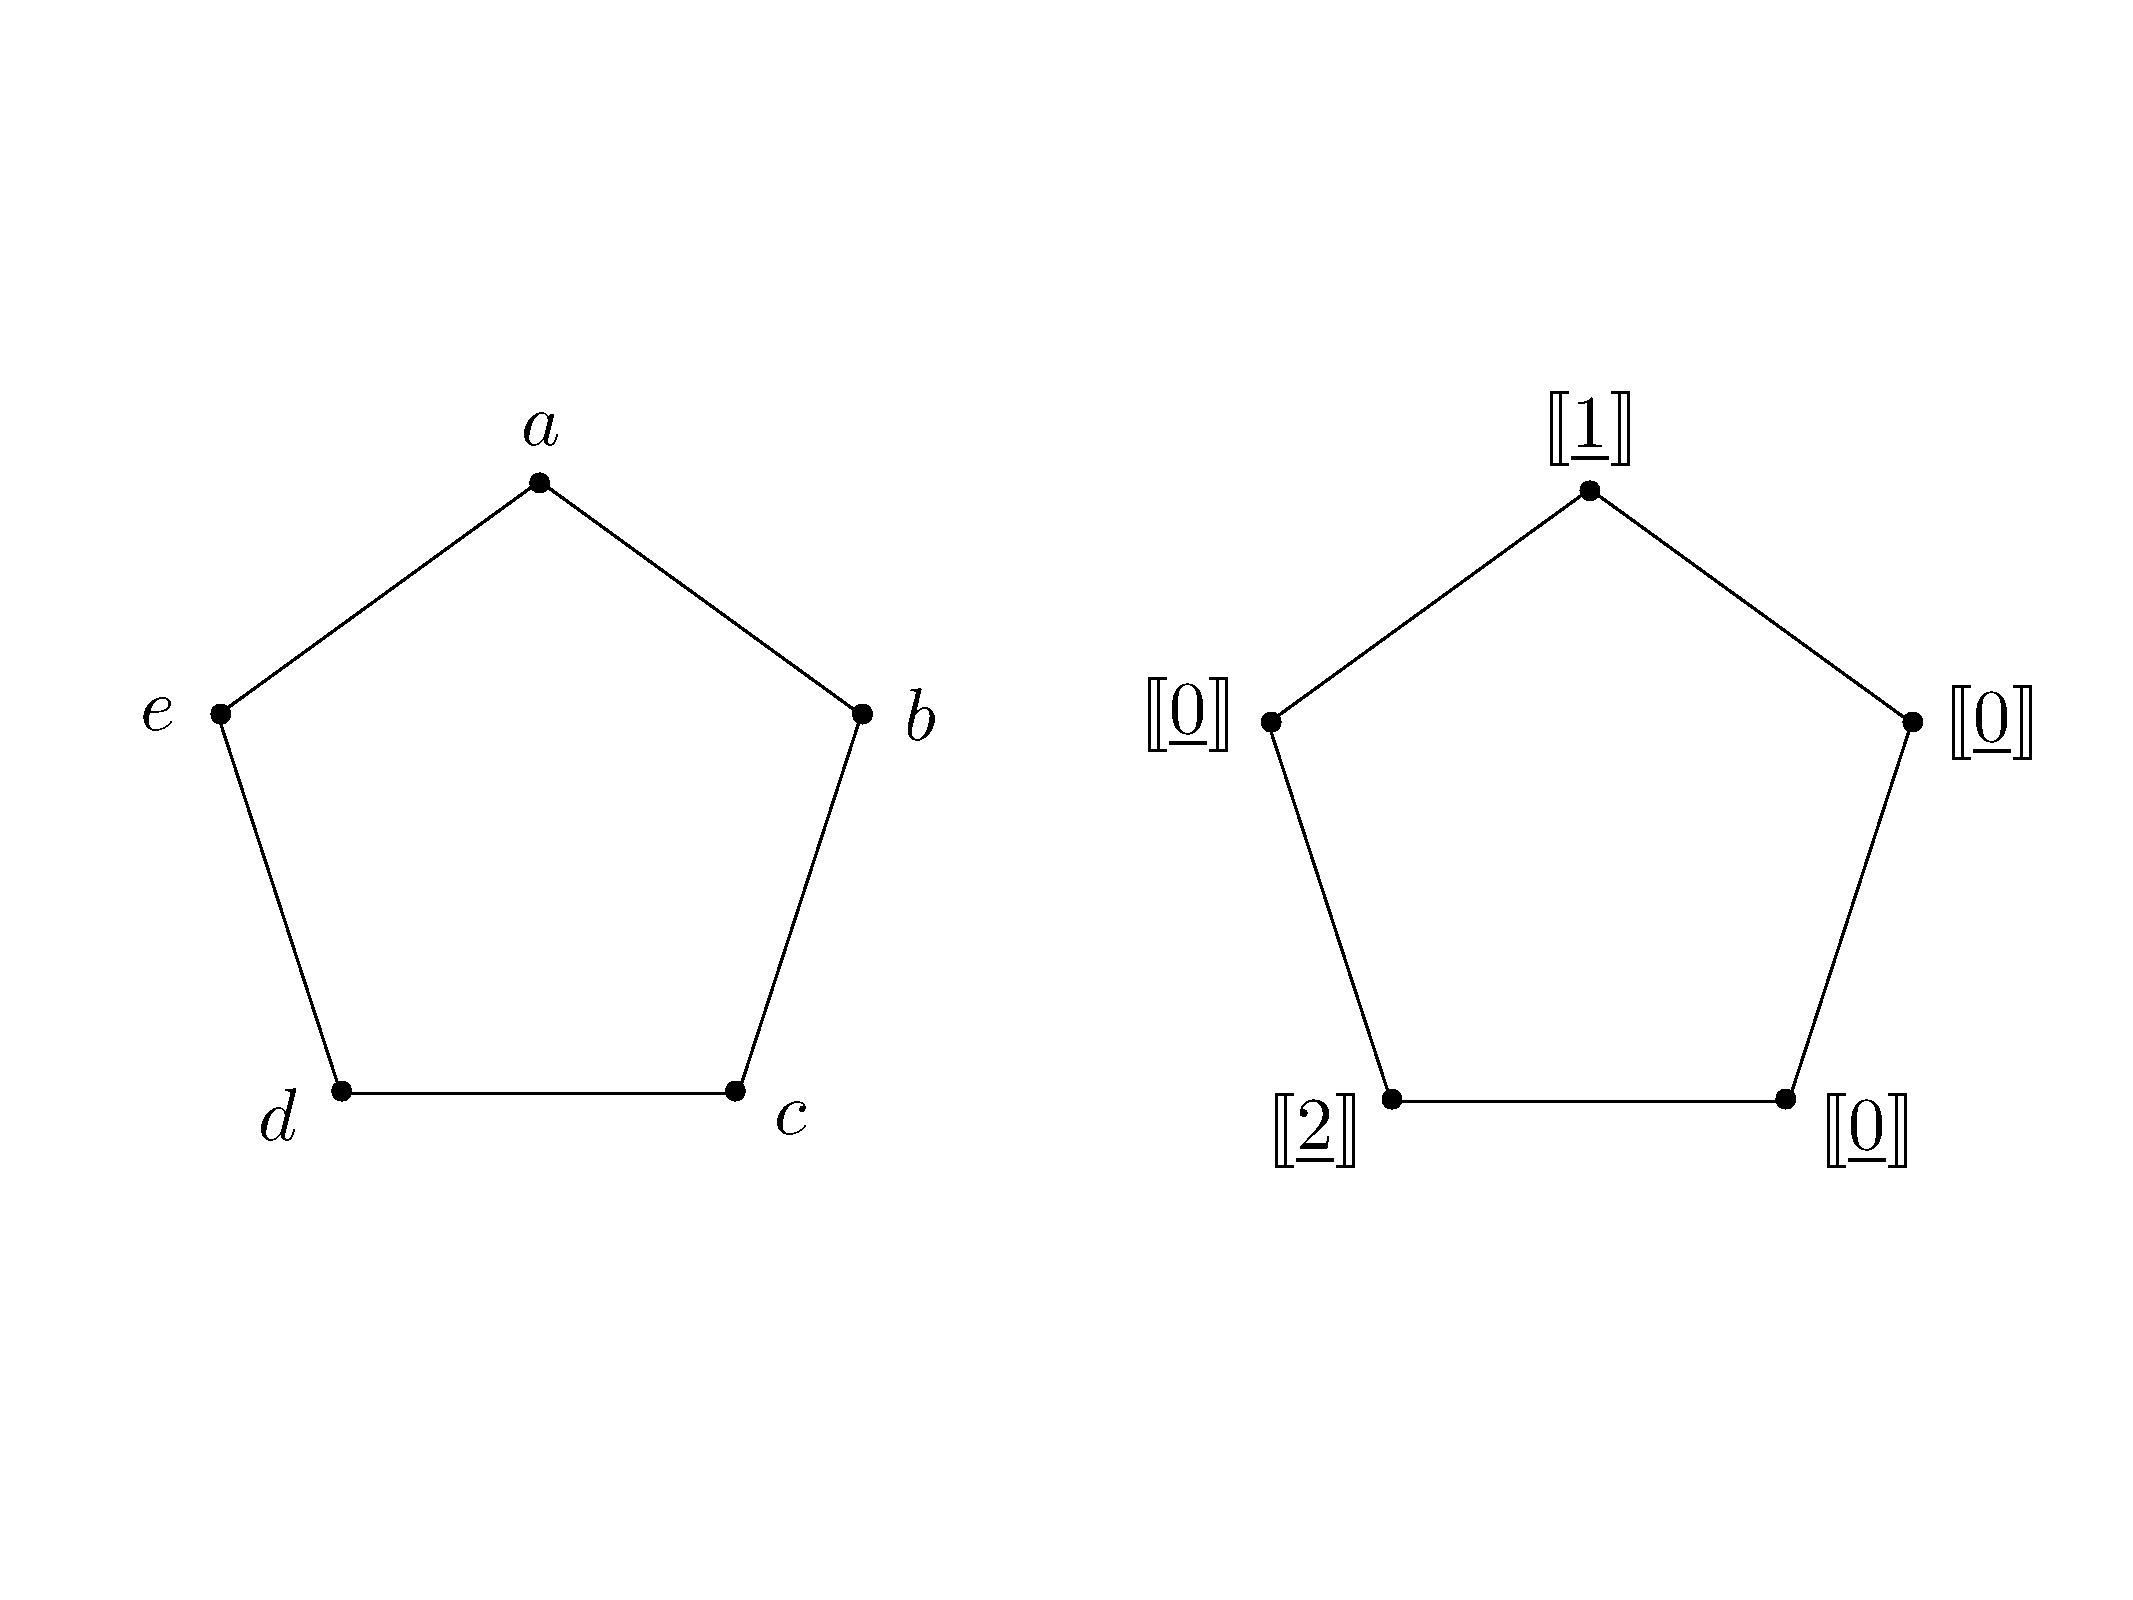
\includegraphics[scale=0.3]{dia2}
\end{center}
and that the state of the third and fourth rings is
\begin{center}
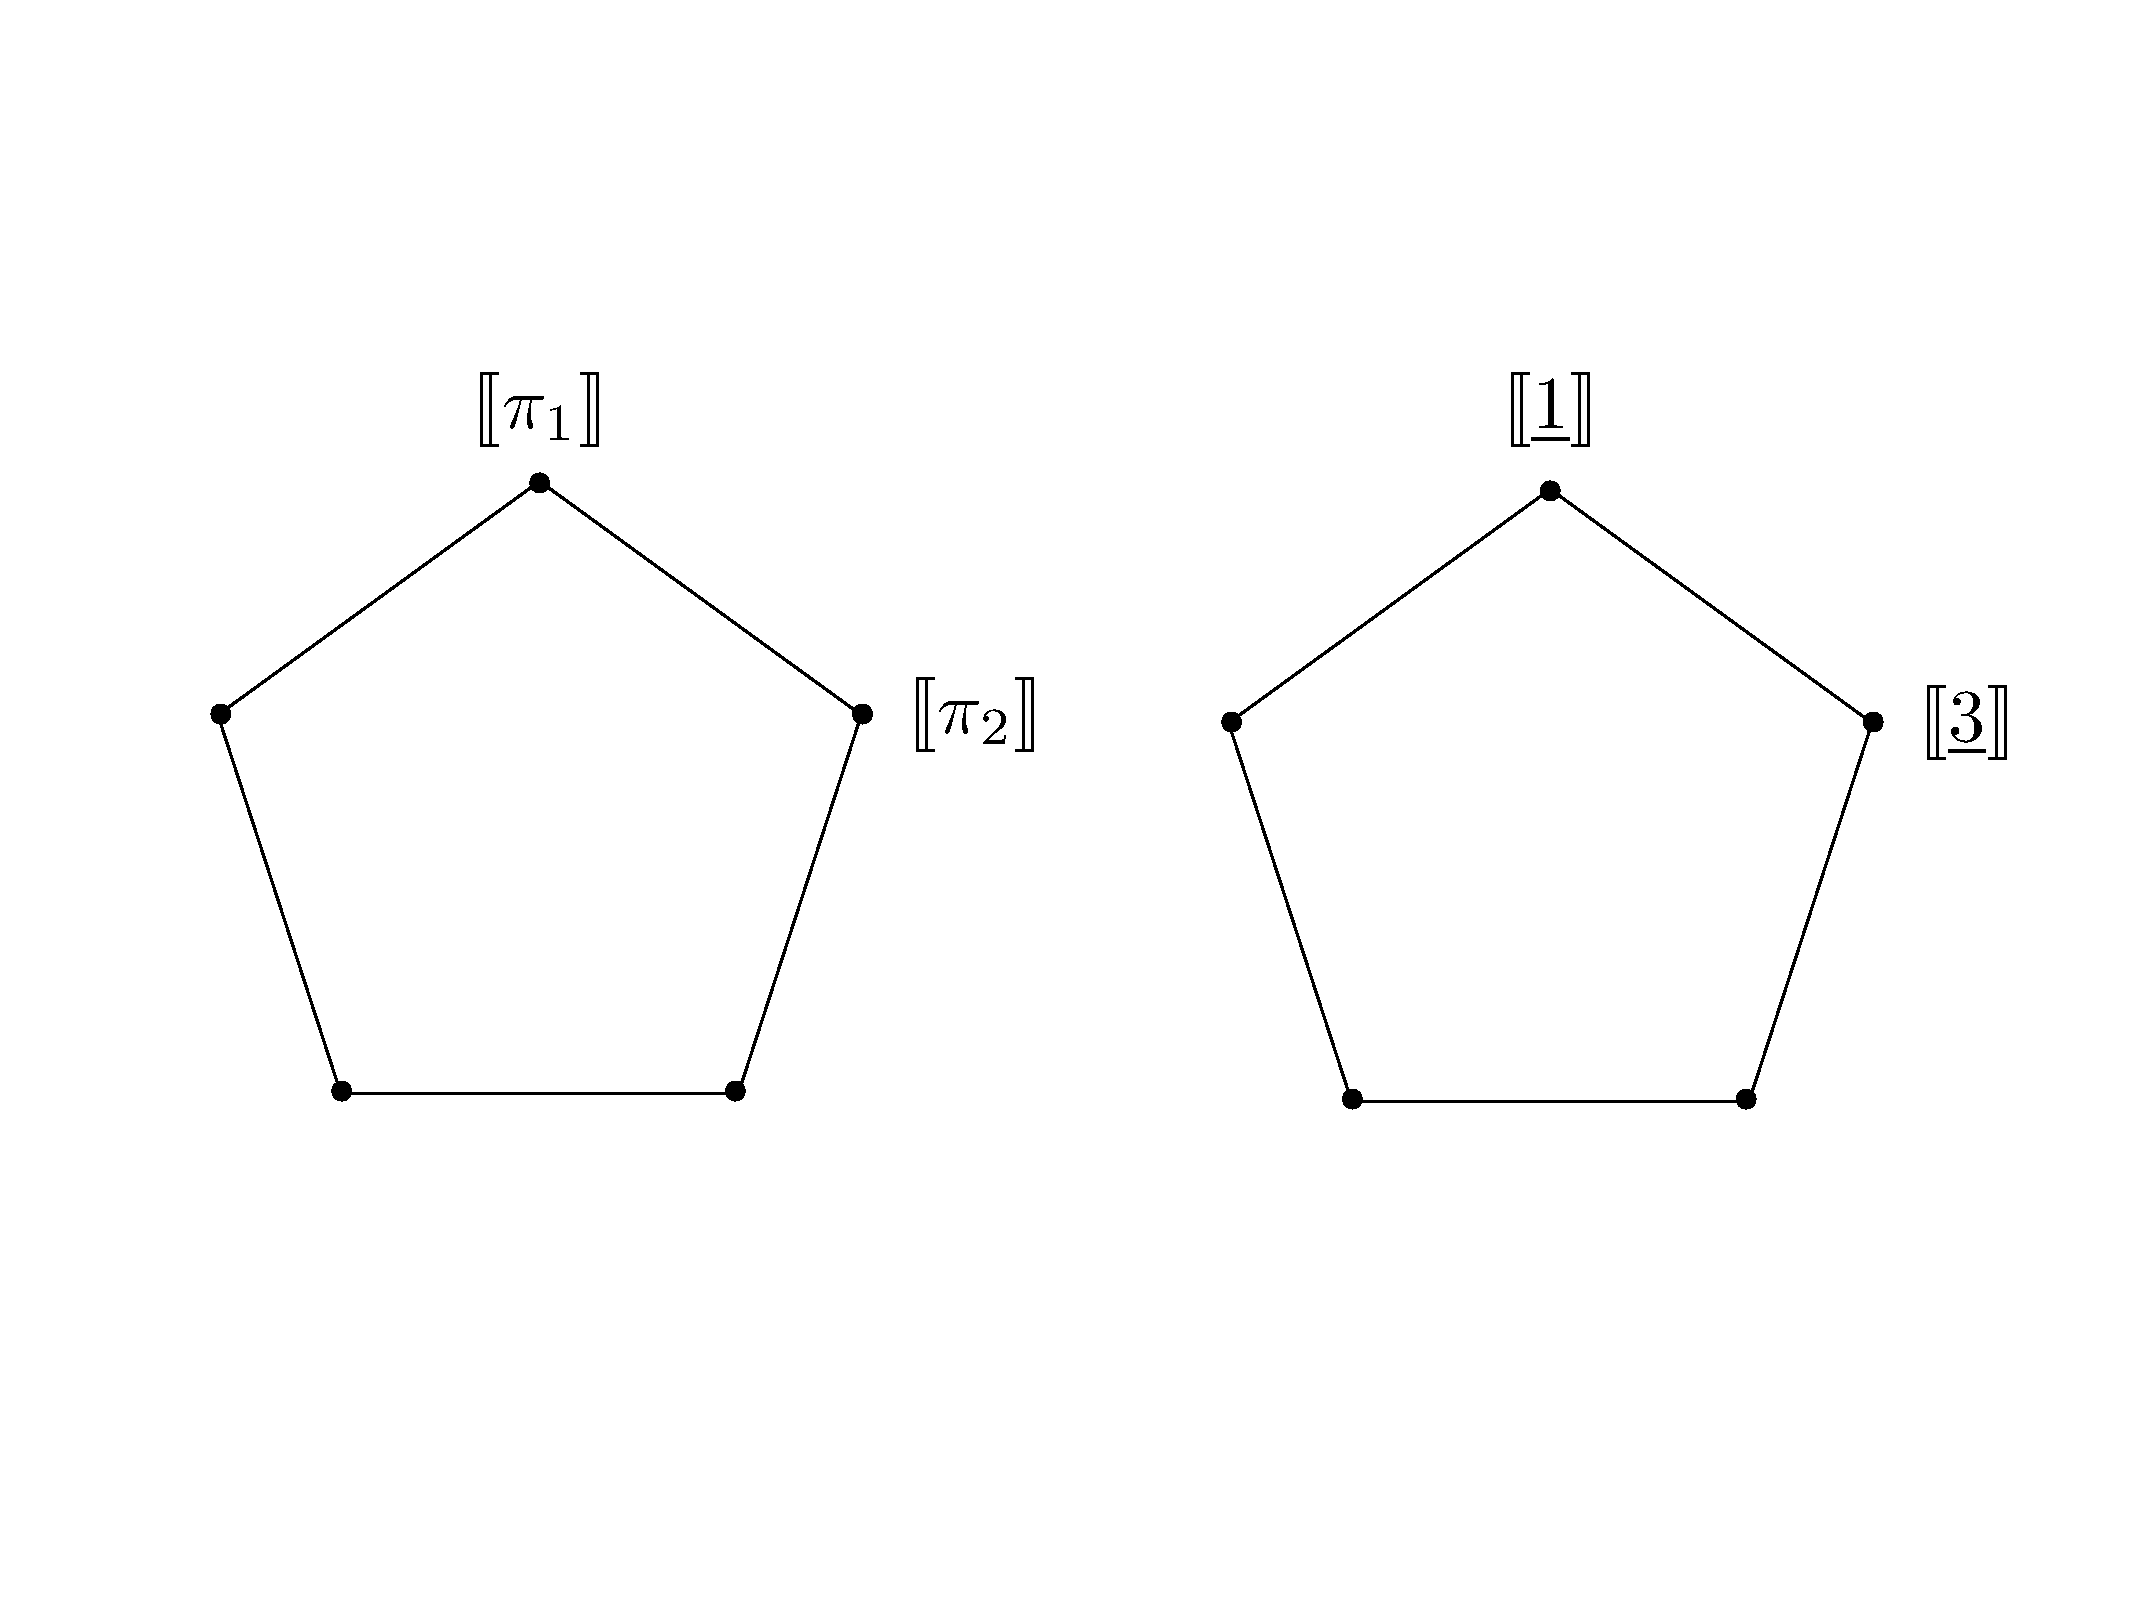
\includegraphics[scale=0.3]{dia3}
\end{center}
Suppose that the read address for the first ring is focused at zero at time $t_0 -1$ and that the focus of the other rings evolves over time according to the table
\begin{center}
\begin{tabular}{|r|c|c|c|c|c|c|c|}
\hline
time after $t_0$ & 0 & 1 & 2 & 3 & 4 & 5 & 6\\
\hline
focus of second ring & 0 & 0 & 1 & 1 & 2 & 1 & 0\\
\hline
focus of third ring & 1 & 0 & 0 & 1 & 1 & 1 & 1\\
\hline
focus of fourth ring & 0 & 0 & 0 & 1 & 0 & 1 & 0\\
\hline
\end{tabular}
\end{center}
At time $t = t_0$ reading from the second, third and fourth rings produces $\den{\underline{2}}, \den{\pi_2}, \den{\underline{1}_{\inta_W}}$ respectively. The controller applies these in reverse order to obtain the iterator
\[
\big\{ \den{\underline{1}_{\inta_W}}( \den{\pi_2} ) \big\}( \den{\underline{2}} ) = \den{\pi_2}( \den{\underline{2}} ) = \den{\underline{4}}\,.
\]
This modified iterator (modified from $\underline{2}$ by the algorithm which is the modification of $\pi_2$ by $\underline{1}_{\inta_W}$) will be the one used by the controller to compute the change in the read address of the first ring from time $t_0 - 1$ to time $t_0$, via the formula
\[
r^{(t_0)} = \den{\underline{4}}_{nl}(R)( r^{(t_0 - 1)} ) = R^4( \overline{0} ) = \overline{4}\,.
\]
This change results in $u_4$ appearing in the computation of $h^{(t_0+1)}$. Using the identity
\begin{gather*}
\big\{\den{\underline{n}_{\inta_W}}_{nl}\big( \den{\pi_k} \big)\big\}\big( \den{\underline{m}_W} \big) = \den{\pi_k}^n( \den{\underline{m}_W} ) = \den{\underline{k^n m}_W}
\end{gather*}
we compute the remaining time steps involve the following iterators:
\begin{align*}
\big\{ \den{\underline{1}_{\inta_W}}_{nl}( \den{\pi_1} ) \big\}( \den{\underline{2}} ) &= \den{\pi_1}( \den{\underline{2}} ) = \den{\underline{2}}\,,\\
\big\{ \den{\underline{1}_{\inta_W}}_{nl}( \den{\pi_1} ) \big\}( \den{\underline{3}} ) &= \den{\pi_1}( \den{\underline{3}} ) = \den{\underline{3}}\,,\\
\big\{ \den{\underline{3}_{\inta_W}}_{nl}( \den{\pi_2} ) \big\}( \den{\underline{3}} ) &= \den{\pi_8}( \den{\underline{3}} ) = \den{\underline{24}}\,,\\
\big\{ \den{\underline{1}_{\inta_W}}_{nl}( \den{\pi_2} ) \big\}( \den{\underline{1}} ) &= \den{\pi_2}( \den{\underline{1}} ) = \den{\underline{2}}\,,\\
\big\{ \den{\underline{3}_{\inta_W}}_{nl}( \den{\pi_2} ) \big\}( \den{\underline{3}} ) &= \den{\pi_8}( \den{\underline{3}} ) = \den{\underline{24}}\,,\\
\big\{ \den{\underline{1}_{\inta_W}}_{nl}( \den{\pi_2} ) \big\}( \den{\underline{2}} ) &= \den{\pi_2}( \den{\underline{2}} ) = \den{\underline{4}}\,.
\end{align*}
The sequence of vectors delivered to the controller will therefore be 
\[
u_0, u_4, u_6 = u_1, u_9 = u_4, u_{33} = u_3, u_{35} = u_0, u_{59} = u_4, u_{63} = u_3.
\]
%When the focus of the fourth ring is at the zero position, the stored proof $\underline{1}_{\inta_W}$ acts on both $\pi_1, \pi_2$ by iterating them once, that is, it does nothing. However, when the focus of the fourth ring is at position one, the stored proof $\underline{3}_{\inta_W}$ at this position iterates any given proof three times, giving respectively $\pi_1, \pi_8$ when fed $\pi_1, \pi_2$. 
Recall that the contents of the second memory ring in the extended NTM appear in the evolution equation via the term $\den{\underline{\mathrm{eval}}}\big( M_2(r_2), \ket{\emptyset}_{\alpha_1} \big)(r_1)$. To define the corresponding term for the current model, we will need the evaluations
\begin{center}
\begin{mathprooftree}
\AxiomC{$\underline{\mathrm{eval}'}$}
\noLine\UnaryInfC{$\vdots$}
\def\extraVskip{5pt}
\noLine\UnaryInfC{$\inta_W \multimap \inta_W, \inta_W \vdash \inta_W$}
\end{mathprooftree}
\qquad
\begin{mathprooftree}
\AxiomC{$\underline{\mathrm{eval}''}$}
\noLine\UnaryInfC{$\vdots$}
\def\extraVskip{5pt}
\noLine\UnaryInfC{$\inta_{\inta_W}, {!}(\inta_W \multimap \inta_W) \vdash \inta_W \multimap \inta_W$}
\end{mathprooftree}
\end{center}
from which we obtain vectors
\begin{gather*}
\den{\underline{\mathrm{eval}}''}( M_4(r_4), \ket{\emptyset}_{M_3(r_3)} ) \in \den{\inta_W \multimap \inta_W}\,,\\
\den{\underline{\mathrm{eval}}'}\Big( \den{\underline{\mathrm{eval}}''}( M_4(r_4), \ket{\emptyset}_{M_3(r_3)} ), M_2(r_2) \Big) \in \den{\inta_W}\,.
\end{gather*}
Since we have four memory rings, the state space of the RNN is decomposed as
\[
\mathscr{H} = \mathscr{H}_0 \oplus \big( \mathscr{W} \oplus \mathscr{W}^* \big)^{\oplus 4}  \oplus \bigoplus_{i=1}^4 \mathscr{S}_i
\]
where $\mathscr{S}_i = \mathscr{W}^* \otimes \mathscr{V}_i$. Using the abbreviations
\[
\Gamma_i = \inta_W, \inta_{W^{\vee}}\,, \qquad \Delta_i = W \multimap W, W^{\vee} \multimap W^{\vee}
\]
the command and data types are given by
\begin{gather*}
\Gamma = \inta_{W^{\vee}}, \Gamma_2, \Gamma_3, \Gamma_4\,\\
\Delta = \Delta_1, \Delta_2, \Delta_3, \Delta_4, V, \inta_W, \inta_W \multimap \inta_W, \inta_{\inta_W}\,.
\end{gather*}
The value of the master function is, for $h = \big(h_0, \{r_i, w_i\}_{i=1}^4, \{M_i\}_{i=1}^4\big)$,
\begin{align*}
\den{\master}_{nl}&\big( \den{\underline{n}_1}, \{\den{\underline{m}_i}, \den{\underline{n}_i}\}_{i=2}^4, \{\alpha_i, \beta_i\}_{i=1}^4, \{u_i\}_{i=1}^4\big)(h)\\
&\quad = \Big(V(M_1(r_1)), \den{\underline{\mathrm{eval}}'}\Big( \den{\underline{\mathrm{eval}}''}( M_4(r_4), \ket{\emptyset}_{M_3(r_3)} ), M_2(r_2) \Big)_{nl}(r_1),\\
&\qquad \beta_1^{n_1}(w_1), \big\{\alpha_i^{m_i}(r_i), \beta_i^{n_i}(w_i)\big\}_{i=2}^4, \big\{M_i + \beta_i^{n_i}(w_i) \otimes u_i \big\}_{i=1}^4 \Big)\,.
\end{align*}
As above we set $\alpha_i = R$ and $\beta_i = R^*$ for $1 \le i \le 4$.

We write $\Phi = \den{\mathrm{less}}$ for the proof of Definition \ref{definition:proofless}.

\begin{lemma}\label{lemma:lessmore} There is a proof $\underline{\mathrm{more}}$ such that denotation gives a linear map
\begin{align*}
\Psi &= \den{\mathrm{more}}: \den{\binta_{W}} \lto \den{\binta_{W \& W}}
\end{align*}
with the following properties:
\begin{itemize}
\item[(i)] $\Phi \circ \Psi = 1$.
\item[(ii)] On the subspace of block matrices
\[
B = \Bigg\{ \begin{pmatrix} \gamma_1 & 0 \\ 0 & \gamma_2 \end{pmatrix} \;\;\Bigg| \;\; \gamma_i \in \End_{\mathbb{R}}(\mathscr{W}) \Bigg\} \subseteq \End_{\mathbb{R}}( \mathscr{W} \oplus \mathscr{W} )
\]
we have
\be
\Psi\big( \den{\underline{S}_W} \big)|_{B \times B} = \den{\underline{S}_{W \& W}}|_{B \times B}
\ee
for all $S \in \{0,1\}^*$.
\end{itemize}
\end{lemma}
\begin{proof}
Let $\pi_i, \iota_i$ denote the projections from and injections into $\den{W \& W} = \mathscr{W} \oplus \mathscr{W}$. We define for $p \in \den{\binta_W}$
\[
\Psi( p )( \alpha, \beta ) = \big( p( \pi_1 \alpha \iota_1, \pi_1 \beta \iota_1 ) , p( \pi_2 \alpha \iota_2, \pi_2 \beta \iota_2 ) \big)\,.
\]
It is clear that this the denotations of a proof. We observe that
\begin{align*}
\big( \Phi \Psi(p) \big)(\alpha, \beta) &= \pi_1 \Psi(p)( \alpha \oplus 1_{\mathscr{W}}, \beta \oplus 1_{\mathscr{W}} )\\
&= \pi_1 \Big( p( \pi_1 (\alpha \oplus 1_{\mathscr{W}}) \iota_1, \pi_1(\beta \oplus 1_{\mathscr{W}}) \iota_1 ), p( \pi_2 (\alpha \oplus 1_{\mathscr{W}}) \iota_2, \pi_2(\beta \oplus 1_{\mathscr{W}}) \iota_2 \Big)\\
&= \pi_1 \big( p(\alpha, \beta), p(1_{\mathscr{W}}, 1_{\mathscr{W}}) \big)\\
&= p(\alpha, \beta)
\end{align*}
which proves (i). It is clear that (ii) holds.
\end{proof}

\subsection{Decaying pattern NTM}

We take the same alphabet $\mathfrak{a}$ as in the multiple pattern NTM, and the same coefficient space $\mathscr{V}_1$ for the first memory ring. There are two additional memory rings, with
\[
\mathscr{V}_2 \subseteq \den{\binta_{W \& W}}\,, \qquad \mathscr{V}_3 \subseteq \den{\binta_{W \& W} \multimap \binta_W \,\&\, \binta_W}\,.
\]
An example of a proof in $\mathscr{V}_3$ is the algorithm $\underline{\mathrm{tail}}$ which takes a binary sequence and returns a pair by separating the tail, for example
\[
\den{\underline{\mathrm{tail}}}\big( \underline{1101}_{W \& W} \big) = (\underline{110}_W, \underline{1}_W)\,.
\]
The idea is that if the third memory ring is sharply focused at $\underline{\mathrm{tail}}$ then we update the second memory ring by replacing a vector $\den{\underline{1101}}$ at a vertex of the ring by its truncation $\den{\underline{110}}$, and we moreover use the tail $\den{\underline{1}}$ to update the first memory ring by reading it as a power of the rotation operator. In this way the contents of the second memory ring \emph{decay} over time. To realise this we need the following auxiliary maps:

\begin{definition}\label{definition:proofless} Given a type $W$ with $\mathscr{W} = \den{W}$ let $\underline{\mathrm{less}}$ be the proof of
\[
\binta_{W \& W} \vdash \binta_W
\]
with the property that for $\alpha, \beta \in \End_{\mathbb{R}}(\den{W})$ and $q \in \den{\binta_{W \& W}}$
\[
\den{\underline{\mathrm{less}}}(q)( \alpha, \beta ) = \pi_1 q( \alpha \oplus 1_{\mathscr{W}}, \beta \oplus 1_{\mathscr{W}} )
\]
where $\pi_i$ denote the projections from $\mathscr{W} \oplus \mathscr{W}$. Then
\[
\Phi \den{\underline{S}_{W \& W}} = \den{\underline{S}_W}
\]
for all $S \in \{0,1\}^*$.
\end{definition}

There does not appear to be a proof $\underline{\mathrm{more}}$ in linear logic which gives a section of $\underline{\mathrm{less}}$ in the sense that its denotation maps $\den{\underline{S}_W}$ to $\den{\underline{S}_{W \& W}}$ (see however Lemma \ref{lemma:lessmore}). But we can just fix one ad hoc (this is simulating second order linear logic in an ugly way).

\begin{definition} We fix a linear map $\psi: \den{\binta_W} \lto \den{\binta_{W \& W}}$ with the property that
\[
\psi \den{\underline{S}_W} = \den{\underline{S}_{W \& W}}
\]
for a finite collection of sequences $S$ that are relevant to the model.
\end{definition}

The master algorithm at a given time step applies $M_3(r_3) \in \mathscr{V}_3$ to $M_2(r_2) \in \mathscr{V}_2$ to get
\[
\den{\feed}( M_2(r_2), M_3(r_3)) \in \den{\binta_W} \oplus \den{\binta_W}\,.
\]
The second component is then applied to the contents of the first memory ring, as in
\[
r_1^{(t+1)} = \Big( \pi_2\den{\feed}( M_2(r_2), M_3(r_3)) \Big)(1_{\mathscr{W}}, R)(r_1^{(t)})\,.
\]
Simultaneously, we update the memory state of the second ring according to the following rule: it becomes the linear map $\mathscr{W} \lto \mathscr{V}_2$ defined by
\[
w \longmapsto \psi \pi_1\den{\feed}( M_2(w), M_3(r_3))\,.
\]
This kind of structure could in principle be used by the controller to predict that an event will happen a fixed amount of time in the future, by pushing ``countdowns'' $\den{\underline{10000}}$ onto the memory ring, and have the controller react to a symbol coming off the first memory ring after it is shifted by the final $\den{\underline{1}}$.

\begin{remark} Actually we seem to have been confused about the kinds of polynomials we get. It seems that unless $\feed$ uses non-linear inputs we never get powers of variables. So we should find an example where this is the case.
\end{remark}